\documentclass[mathserif,16pt,xcolor=table]{beamer}

% Load Beamer Style Theme
% TAMU Based
\usepackage{tamu_beamer}
% \usepackage[skip=0pt]{caption}

% Specifiy the location of images to be used
\graphicspath{{figures/}}

% ------------------------------------------------------------
% ------------------------------------------------------------
% ------------------------------------------------------------
% ----------------TITLE PAGE----------------------------------
% ------------------------------------------------------------
% ------------------------------------------------------------
% ------------------------------------------------------------
% Document Title Page
\title{Surface wave supporting structures in the terahertz and optical frequency domains}
% \subtitle{Preliminary Exam}
\author[Hasan Tahir Abbas]{Hasan Tahir Abbas\\~\\{\small {Supervised by: Dr. Robert D. Nevels}}}
\institute{Department of Electrical  \& Computer Engineering\\ \mbox{} \\ \pgfuseimage{tamuecenbig}}
\date[Summer 2017]{\today}
% ------------------------------------------------------------
% ------------------------------------------------------------
% ------------------------------------------------------------
% ------------------------------------------------------------
% ------------------------------------------------------------
% ------------------------------------------------------------
% ------------------------------------------------------------
% ------------------------------------------------------------
% ------------------------------------------------------------
% ------------------------------------------------------------
% ------------------------------------------------------------
% ------------------------------------------------------------
% ------------------------------------------------------------
% ------------------------------------------------------------
\begin{document}

% Reduce space around equations and subequations
\preto\subequations{\ifhmode\unskip\fi}
\AtBeginEnvironment{subequations}{\ifhmode\unskip\fi}
\AtBeginEnvironment{equation}{\ifhmode\unskip\fi}

% Draw Boxes in the footer with pertinent info
\tikzstyle{block} = [rectangle, draw, rounded corners, shade, top color=white, text width=5em,
bottom color=blue!50!black!20, draw=blue!40!black!60, very thick, text centered, minimum height=4em]
\tikzstyle{line} = [draw, -latex']
\tikzstyle{cloud} = [draw, ellipse,top color=white, bottom color=red!20, node distance=2cm, minimum height=2em]

% Tick Style
\beamertemplateballitem
% \beamertemplatetransparentcoveredhigh

\frame{\titlepage}


% Add TAMU logo on each slide in the north-east side
% Shifted to be right at the edge
%
% NOTE: Will have to compile twice
%
\addtobeamertemplate{frametitle}{}{%
\begin{tikzpicture}[remember picture,overlay]
  \node[anchor=north east,yshift=7pt,xshift=2pt] at (current page.north east) {
\includegraphics[height=.7cm]{ecen}};
\end{tikzpicture}}
% ------------------------------------------------------------
% ------------------------------------------------------------
% ------------------------------------------------------------
% ------------------------------------------------------------
% ------------------------------------------------------------
% ------------------------------------------------------------
% ------------------------------------------------------------
% ------------------------------------------------------------
% ------------------------------------------------------------
% ------------------------------------------------------------
% ------------------------------------------------------------
% ------------------------------------------------------------
% ------------------------------------------------------------
% ------------------------------------------------------------
\section{Outline}
\begin{frame}
  \frametitle{Outline}
  \begin{outline}[itemize]
    \1 Overview
    \1 Background
    \1 Theory and Methods
    \2 Sommerfeld Integral analysis
    \2 Dispersion relation
    \2 Surface Integral equation
    \1 Results
    \2 Super-resolution Imaging
    \1 Conclusions
  \end{outline}
\end{frame}
% ------------------------------------------------------------
% ------------------------------------------------------------
% ------------------------------------------------------------
% ------------------------------------------------------------
% ------------------------------------------------------------
% ------------------------------------------------------------
% ------------------------------------------------------------
% ------------------------------------------------------------
% ------------------------------------------------------------
% ------------------------------------------------------------
% ------------------------------------------------------------
% ------------------------------------------------------------
% ------------------------------------------------------------
\section{Overview}
% ------------------------------------------------------------
% ------------------------------------------------------------
\begin{frame}
  \frametitle{Overview}
  % ----------------------------------------------------------
  % Talk about the significance of this research
  \begin{columns} % align columns
    \begin{column}{.5\textwidth} \vspace*{-1cm}
      \begin{outline}[itemize]
        \1 Plasmonics: subwavelength localization of electromagnetic (EM) fields
        \1 Plasma frequency
        \2 Metals - Optical frequency
        \2 2D Electronic Systems (2DES) - Terahertz (THz)
        \1 Bridging the THz gap
      \end{outline}
    \end{column}
    \begin{column}{.5\textwidth}
      % Use this to preserve fonts from Inkspace
      \begin{figure}
        \centering \hspace*{-0.75cm}
        \fontsize{6}{7}\selectfont
        \def\svgwidth{1.1\linewidth}
        \input{figures/scale.pdf_tex}
        \label{fig:spp_2deg}
        \caption{Communication Technologies at various frequencies}
      \end{figure}
      \end{column}%
    \end{columns}
  \end{frame}
  % ------------------------------------------------------------
  % ------------------------------------------------------------
  % ------------------------------------------------------------
  % ------------------------------------------------------------
  % ------------------------------------------------------------
  % ------------------------------------------------------------
  % ------------------------------------------------------------
  % ------------------------------------------------------------
  % ------------------------------------------------------------
  \begin{frame}
    \frametitle{Overview}
    \framesubtitle{Terahertz 2DES}
    % ----------------------------------------------------------
    % Talk about the significance of this research
    \begin{outline}[itemize]
      \1 Graphene
      \2 Grown separately, transfered to substrate
      \2 Currently not integrable to current electronics technology
      \2 Superior electronic properties
      \1 Semiconductor heterostructures
      \2 Conventional epitaxial semiconductor device fabrication techniques
      \2 On-chip integration with silicon electronics
    \end{outline}
  \end{frame}

  % ------------------------------------------------------------
  % ------------------------------------------------------------
  % ------------------------------------------------------------
  % ------------------------------------------------------------
  % ------------------------------------------------------------
  % ------------------------------------------------------------
  % ------------------------------------------------------------

  % ------------------------------------------------------------
  % ------------------------------------------------------------
  % ------------------------------------------------------------
  % ------------------------------------------------------------
  % ------------------------------------------------------------
  % ------------------------------------------------------------
  % ------------------------------------------------------------
  \section{Background}
  % ------------------------------------------------------------
  % ------------------------------------------------------------
  % ------------------------------------------------------------
  % ------------------------------------------------------------
  % ------------------------------------------------------------
  % ------------------------------------------------------------
  % ------------------------------------------------------------
  % ------------------------------------------------------------
  % ------------------------------------------------------------
  % ------------------------------------------------------------
  % ------------------------------------------------------------
  % ------------------------------------------------------------
  % ------------------------------------------------------------
  \begin{frame}
    \frametitle{Background}
    \framesubtitle{Plasmonics Overview}
    % ----------------------------------------------------------
    \begin{columns} % align columns
      \begin{column}{.5\textwidth}
        \begin{outline}[itemize]
          \1 Interfacial wave phenomena
            \2 Metal-dielectric interface
            \2 Semiconductor heterostructure
          \1 Surface plasmon polaritons (SPPs)
        \end{outline}
        %
        \begin{outline}[itemize]
          \1 Plasma frequency
          \2 Metals - Optical frequency
          \2 Semiconductors - Terahertz
        \end{outline}
        %
      \end{column}
      \begin{column}{.5\textwidth}
        % Use this to preserve fonts from Inkspace
        \begin{figure}
          \centering
          \fontsize{6}{7}\selectfont% Reduce the fontsize
          \def\svgwidth{.8\linewidth}
          \input{figures/spp.pdf_tex}
          \label{fig:spp}
          \caption{SPPs at optical frequencies}
        \end{figure}
        %
        \begin{figure}
          \centering
          \fontsize{6}{7}\selectfont
          \def\svgwidth{.8\linewidth}
          \input{figures/spp_2deg.pdf_tex}
          \label{fig:spp_2deg}
          \caption{SPPs in the THz regime}
        \end{figure}
        \end{column}%
      \end{columns}
    \end{frame}
    % ------------------------------------------------------------
    % ------------------------------------------------------------
    % ------------------------------------------------------------
    % ------------------------------------------------------------
    % ------------------------------------------------------------
    % ------------------------------------------------------------
    % ------------------------------------------------------------
    \begin{frame}
      \frametitle{Background}
      \framesubtitle{Surface Plasmon Polaritons}

      \begin{columns} % align columns
        \begin{column}{.5\textwidth}
          \begin{minipage}[T][.1\textheight][c]{\linewidth}
            \begin{outline}[itemize]
              \1 Slow surface waves
              \1 Reduced Wavelength
              \1 Focusing beyond the diffraction limit
            \end{outline}
            \begin{outline}[itemize]
              \1 Optical SPP
            \end{outline}
            \setlength{\belowdisplayshortskip}{-7pt}
            \setlength{\abovedisplayshortskip}{2pt}
            \begin{equation} \nonumber
              \Re \left[ \E_{\text{metal}}(\O)\right] < 0
            \end{equation}
            \begin{outline}[itemize]
              \1 THz SPP
            \end{outline}
            \begin{equation} \nonumber
              \Im \left[ \sigma_{s}(\O)\right] < 0
            \end{equation}
          \end{minipage}
        \end{column}
        \begin{column}{.5\textwidth}
          % Use this to preserve fonts from Inkspace
          \begin{figure}
            \centering \hspace*{-1.25cm}
            \fontsize{6}{7}\selectfont
            \def\svgwidth{1.1\linewidth}
            \input{figures/spps_comp.pdf_tex}
            \label{fig:spp_2deg}
            \caption{Dispersion Curve comparison}
          \end{figure}
          \end{column}%
        \end{columns}
      \end{frame}
      % ------------------------------------------------------------
      % ------------------------------------------------------------
      % ------------------------------------------------------------
      % ------------------------------------------------------------
      % ------------------------------------------------------------
      % ------------------------------------------------------------
      % ------------------------------------------------------------
      % ------------------------------------------------------------
      \begin{frame}
        \frametitle{Background}
        \framesubtitle{Optical Nanoantennas}

        \begin{columns} % align columns
          \begin{column}{.45\textwidth}
            % \begin{minipage}[T][.1\textheight][c]{\linewidth}
            \vspace*{-1cm}
              \begin{outline}[itemize]
                \1 Convert Localized near-field to efficient far-field radiation
                \1 Low Q-factor
                \1 Extremely small size
                \1 \color{red}{High Purcell Factor}
              \end{outline}
              % \setlength{\belowdisplayshortskip}{-7pt}
              % \setlength{\abovedisplayshortskip}{2pt}
            \begin{equation} \nonumber
              {P}  = \frac{{Q}}{{V}}
            \end{equation}
            \begin{outline}[itemize]
              \1 Directive radiation
            \end{outline}
            % \end{minipage}
            %
          \end{column}
          %
          \begin{column}{.55\textwidth}
            \vspace*{-1cm}
            % Use this to preserve fonts from Inkspace
            \begin{figure}
              \centering \hspace*{-1.25cm}
              \fontsize{6}{7}\selectfont
              \def\svgwidth{1.1\linewidth}
              \input{figures/curto.pdf_tex}
              \caption{Optical resonant cavities for electric field enhancement}
            \end{figure}
            \end{column}%
          \end{columns}
        \end{frame}
      %   % ------------------------------------------------------------
      %   % ------------------------------------------------------------
      %   % ------------------------------------------------------------
      %   % ------------------------------------------------------------
      %   % ------------------------------------------------------------
      %   % ------------------------------------------------------------
      %   % ------------------------------------------------------------
      %   % ------------------------------------------------------------
        \begin{frame}
          \frametitle{Background}
          \framesubtitle{Optical Nanoantennas (contd.)}

          \begin{columns} % align columns
            \begin{column}{.45\textwidth}
              \begin{minipage}[T][.1\textheight][c]{\linewidth}
                \begin{outline}[itemize]
                  \1 Scaled-down microwave antenna designs
                    \2 Aperture antennas for subwavelength focusing
                    \2 Broadband spectral response : Bowtie
                \end{outline}
                \begin{figure}
                  \includegraphics[scale=.03]{bowtie_field_map.png}
                  % \caption{Subwavelength Transmission through a Silver slit}
                \end{figure}
              \end{minipage}
            \end{column}
            %
            \begin{column}{.55\textwidth}
              % Use this to preserve fonts from Inkspace
              \vspace*{-1.5cm}
              \begin{figure}
                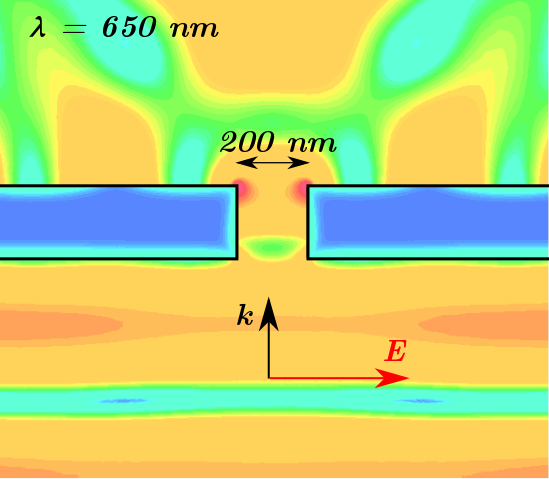
\includegraphics[scale=.2]{E_squared_final.png}
              \end{figure}
              \vspace*{-1cm}
              \begin{figure} \hspace*{-.25cm} \centering
                \includegraphics[width = 1.05\linewidth]{fig13.jpg}
                \label{fig:cst_simulation}
              \end{figure}
              \end{column}%
            \end{columns}
          \end{frame}
      %     % ------------------------------------------------------------
      %     % ------------------------------------------------------------
      %     % ------------------------------------------------------------
      %     % ------------------------------------------------------------
      %     % ------------------------------------------------------------
      %     % ------------------------------------------------------------
      %     % ------------------------------------------------------------
      %     % ------------------------------------------------------------
          \begin{frame}
            \frametitle{Background}
            \framesubtitle{Two-dimensional Electron Gas (2DEG)}

            \begin{columns} % align columns
              \begin{column}{.5\textwidth}
                \begin{minipage}[T][.1\textheight][c]{\linewidth}
                  \begin{outline}[itemize]
                    \1 Semiconductor Heterostructure in high electron mobility transistor (HEMT)
                    \1 High concentration of free electrons ($\sim \num{1e12}-\SI{1e14}{\cm^{-2}}$)
                    \1 Very high Mobility ($\sim \num{1e4}-\SI{1e6}{\cm^{2}/V/s}$)
                    \1 Formation of Quantum Well
                      \2 Two-dimensional confinement of electrons
                  \end{outline}
                \end{minipage}
                %
              \end{column}
              %
              \begin{column}{.5\textwidth}
                % Use this to preserve fonts from Inkspace
                \begin{figure}
                  \centering
                  \fontsize{6}{7}\selectfont
                  \def\svgwidth{.8\linewidth}
                  \input{figures/hemt2.pdf_tex}
                  \caption{Typical GaAs/AlGaAs HEMT}
                \end{figure}
                \begin{figure}
                  \centering \vspace*{-1cm}
                  \fontsize{6}{7}\selectfont
                  \def\svgwidth{.8\linewidth}
                  \input{figures/2deg_bandgap.pdf_tex}
                  \caption{Band diagram of a GaAs/AlGaAs heterostructure}
                \end{figure}
                \end{column}%
              \end{columns}
            \end{frame}
      %       % ------------------------------------------------------------
      %       % ------------------------------------------------------------
      %       % ------------------------------------------------------------
      %       % ------------------------------------------------------------
      %       % ------------------------------------------------------------
      %       % ------------------------------------------------------------
      %       % ------------------------------------------------------------
      %       % ------------------------------------------------------------
            \begin{frame}
              \frametitle{Background}
              \framesubtitle{2DEG (contd.)}

              \begin{columns} % align columns
                \begin{column}{.5\textwidth}
                  \begin{minipage}[T][.1\textheight][c]{\linewidth}
                    \begin{outline}[itemize]
                      \1 Plasma waves in 2DEG
                      \1 Dyakonov-Shur instability
                        \2 Voltage bias at source and drain terminals
                        \2 Plasma resonance
                        \2 THz emission
                      \1 Electronic Flute
                        \2 Tunable resonance with gate voltage
                      \1 Shallow water waves
                    \end{outline}
                  \end{minipage}
                  %
                \end{column}
                %
                \begin{column}{.5\textwidth}
                  % Use this to preserve fonts from Inkspace
                  \begin{figure}
                    \hspace*{-.55cm}
                    \fontsize{6}{7}\selectfont
                    \def\svgwidth{1.1\linewidth}
                    \input{figures/flute_2deg2.pdf_tex}
                    % \caption{Typical GaAs/AlGaAs HEMT}
                  \end{figure}
                  \begin{equation} \nonumber
                    \begin{split}
                      \lambda &= \frac{c}{f} \\
                      & \Longrightarrow  300 \u \mathrm{m}
                    \end{split}
                    \label{eq:disp_TE_two}
                  \end{equation}
                  \end{column}%
                \end{columns}
              \end{frame}
      %         % ------------------------------------------------------------
      %         % ------------------------------------------------------------
      %         % ------------------------------------------------------------
      %         % ------------------------------------------------------------
      %         % ------------------------------------------------------------
      %         % ------------------------------------------------------------
      %         % -------------------THEORY-----------------------------------
      %         % ------------------------------------------------------------
      %         % ------------------------------------------------------------
      %         % ------------------------------------------------------------
      %         % ------------------------------------------------------------
      %         % ------------------------------------------------------------
      %         % ------------------------------------------------------------
      %         % ------------------------------------------------------------
      %         % ------------------------------------------------------------
      %         % ------------------------------------------------------------
      %         % Beginning of the actual content
      \section{Theory and Methods}
      % \begin{frame}
      %   \frametitle{Theory}
      %   \framesubtitle{SPP Dispersion Relation}
      %   \begin{columns}[T] % align columns
      %     \begin{column}{.5\textwidth}
      %       \begin{outline}[itemize]
      %         \1 SPP pole
      %       \end{outline}
      %       \begin{equation} \nonumber
      %         k_{sp}=\frac{\O}{c}\sqrt {\dfrac {\E_{1}\E_{2}(\O)} {\E_{1} + \E_{2}(\O)}}
      %         \label{eq:dis_spp}
      %       \end{equation}
      %       \begin{outline}[itemize]
      %         \1 Accurate material description
      %       \end{outline}
      %       \begin{equation} \nonumber
      %         \E_2(\O) = \E_{\inf} - \frac{\O_{d}^{2}}{\O^2 - \j\gamma \O} + \sum \limits_{i = 1}^N G_i(\O)
      %         \label{eq:eps_drude_cp}
      %       \end{equation}
      %       \begin{equation} \nonumber
      %         G_i(\O) = C_i \left[ \frac{e^{\j \phi_i}}{\O_i + \O - \j \Gamma_i} + \frac{e^{-\j \phi_i}}{\O_i - \O + \j \Gamma_i} \right]
      %         \label{eq:CP_terms}
      %       \end{equation}
      %     \end{column}
      %     \begin{column}[T]{.45\textwidth}
      %       \vspace*{-2cm}
      %       \centering
      %       \begin{figure}
      %         \subfloat{\includegraphics[height = 1.5in]{ep_silver.tikz}
      %         \label{fig:ep_gold}}
      %
      %         \subfloat{\hspace*{-.1cm} \includegraphics[height = 1.5in]{disp_silver.tikz}
      %         \label{fig:ep_silver}}
      %       \end{figure}
      %     \end{column}
      %   \end{columns}
      % \end{frame}
      %     % ------------------------------------------------------------
      %     % ------------------------------------------------------------
      %     % ------------------------------------------------------------
      %     % ------------------------------------------------------------
      %     % ------------------------------------------------------------
      %     % ------------------------------------------------------------
      %     % ------------------------------------------------------------
      \begin{frame}
        \frametitle{Theory and Methods}
        \framesubtitle{2DEG Circuit model}
        \begin{columns} % align columns
          \begin{column}{.5\textwidth}
            \begin{minipage}[T][.1\textheight][c]{\linewidth}
              \begin{outline}[itemize]
                \1 Drude-Lorentz Surface Conductivity
              \end{outline}
              %
              \begin{equation} \nonumber
                \sigma_s = \frac{N_s e^2}{m^{\ast}}\frac{\tau}{1 + \j \tau \O}
                \label{eq:Y2deg}
              \end{equation}
              \begin{itemize}
                \item[] {\makebox[.3cm][l]{$N_s$} - Surface charge density}
                \item[] {\makebox[.3cm][l]{$\tau$} - Scattering time}
                \item[] {\makebox[.3cm][l]{$m^{\ast}$} - Effective electron mass}
              \end{itemize}
              \begin{outline}[itemize]
                \1 Equivalent Circuit
                \end{outline}
                \begin{equation} \nonumber
                  \sigma_s = \frac{1}{Z} = \frac{1}{R + {1}/{\j \O C}}
                  \label{eq:simga_TL}
                \end{equation}
            \end{minipage}
          \end{column}
          %
          \begin{column}{.5\textwidth}
            % Use this to preserve fonts from Inkspace
            \begin{figure} \vspace*{-1.75cm}
              \includegraphics[height = 2.0in]{cond_2deg_gan.tikz}
              \label{fig:cond_2deg}
              \caption{Room temperature GaN/AlGaN 2DEG surface conductivity}
            \end{figure}
            %
            \begin{figure} \vspace*{-.75cm}
              \centering
              \fontsize{6}{7}\selectfont
              \def\svgwidth{.75\linewidth}
              \input{figures/circuit.pdf_tex}
              % \caption{Typical GaAs/AlGaAs HEMT}
            \end{figure}
            \end{column}%
          \end{columns}
        \end{frame}
      %           % ------------------------------------------------------------
      %           % ------------------------------------------------------------
      %           % ------------------------------------------------------------
      %           % ------------------------------------------------------------
      %           % ------------------------------------------------------------
      %           % ------------------------------------------------------------
      %           % ------------------------------------------------------------
      \begin{frame}
        \frametitle{Theory and Methods}
        \framesubtitle{Dispersion Relation for a 2D Sheet}
        \begin{columns}[T] % align columns
          \begin{column}{.5\textwidth}
            \begin{outline}[itemize]
              \1 Conductive Sheet in freespace
              \1 TM mode surface wave
            \end{outline}
            \begin{equation} \nonumber
              k^{\mathrm{TM}}_{\mathrm P} = \frac{\O}{c} \sqrt{1 - \left(\frac{2}{\eta_0 \sigma_s}\right)^2}
              \label{eq:TM_pole}%
            \end{equation}
            \begin{outline}[itemize]
              \1 Below plasma frequency
              \end{outline}
            \begin{equation} \nonumber
              \Im \sigma_s < 0
              \label{eq:2deg_surface_wave}%
            \end{equation}%
            \begin{outline}[itemize]
              \1 At low temperature
              \end{outline}%
            \begin{equation} \nonumber
              \Im |\sigma_s| \gg \Re |\sigma_s|
              \label{eq:2deg_low_loss}
            \end{equation}
          \end{column}
          \begin{column}[T]{.45\textwidth}
            \vspace*{-2cm}
            \centering
            \begin{figure}
              \subfloat{\includegraphics[height = 1.5in]{disp_gaas_sheet_77.tikz}
              \label{fig:disp_2deg_77}}

              \subfloat{\hspace*{-.1cm} \includegraphics[height = 1.5in]{disp_gaas_sheet_rt.tikz}
              \label{fig:disp_2deg_rt}}
            \end{figure}
          \end{column}
        \end{columns}
      \end{frame}
      %           % ------------------------------------------------------------
      %           % ------------------------------------------------------------
      %           % ------------------------------------------------------------
      %           % ------------------------------------------------------------
      %           % ------------------------------------------------------------
      %           % ------------------------------------------------------------
      %           % ------------------------------------------------------------
      \begin{frame}
        \frametitle{Theory and Methods}
        \framesubtitle{Analyzing multilayer structure}
        \begin{columns}[T] % align columns
          \begin{column}{.45\textwidth}
            \begin{outline}[itemize]
              \1 Equivalent transmission line (TL) network
              \1 Dispersion relation
                \2 Transverse resonance condition
            \end{outline}
            \begin{equation} \nonumber
              Y^{\uparrow}(z_0) + Y^{\downarrow}(z_0) + Y_{\sigma} = 0.
              \label{eq:dispersion}
            \end{equation}
            \begin{outline}[itemize]
              \1 Below plasma frequency
              \end{outline}
          \end{column}
          \begin{column}[T]{.65\textwidth}
            \vspace*{-1cm} \hspace*{-2cm}
            \begin{figure}
              \centering \hspace*{-.5cm}
              \fontsize{6}{7}\selectfont
              \def\svgwidth{1.2\linewidth}
              \input{figures/mlayers.pdf_tex}
              % \caption{Typical GaAs/AlGaAs HEMT}
            \end{figure}
          \end{column}
        \end{columns}
      \end{frame}
      %           % ------------------------------------------------------------
      %           % ------------------------------------------------------------
      %           % ------------------------------------------------------------
      %           % ------------------------------------------------------------
      %           % ------------------------------------------------------------
      %           % ------------------------------------------------------------
      %           % ------------------------------------------------------------
      %           \begin{frame}[t]
      %             \frametitle{Nanoscale Imaging scheme}
      %             \framesubtitle{Basics}
      %             \begin{columns}[T] % align columns
      %               \begin{column}{.4\textwidth}
      %                 \begin{outline}[itemize]
      %                   \1 Structured Illumination
      %                   \2 Periodic sine pattern
      %                   \1 Moiré Fringes
      %                   \2 Frequency modulation of two patterns
      %                   \2 Resulting low-frequency signal
      %                   \1 Linear scheme
      %                   \2 Low light intensity
      %                 \end{outline}
      %               \end{column}
      %               %%
      %               %%
      %               \begin{column}[T]{.6\textwidth}
      %                 \begin{center}
      %                   \begin{figure}[t!]
      %                     \vspace*{-2cm}
      %                     \centering
      %                     \subfloat{\scalebox{.07}{\input{figures/fine_lines.pdf_tex}}
      %                     \label{fig:test}} \hfil
      %                     \subfloat{\scalebox{.07}{\input{figures/fine_lines_2.pdf_tex}}
      %                     \label{fig:sim_hi}}
      %                   \end{figure}
      %                   \begin{figure}
      %                     \vspace*{-.5cm}
      %                     \centering
      %                     \def\svgwidth{.6\linewidth}
      %                     \input{figures/fine_lines_moire.pdf_tex}
      %                   \end{figure}
      %                 \end{center}
      %                 \end{column}%
      %               \end{columns}
      %             \end{frame}
      %             % ------------------------------------------------------------
      %             % ------------------------------------------------------------
      %             % ------------------------------------------------------------
      %             % ------------------------------------------------------------
      %             % ------------------------------------------------------------
      %             % ------------------------------------------------------------
      %             % ------------------------------------------------------------
      %             % ------------------------------------------------------------
      %             % ------------------------------------------------------------
      %             % ------------------------------------------------------------
      %             % ------------------------------------------------------------
      %             % ------------------------------------------------------------
      %             % ------------------------------------------------------------
      %             % ------------------------------------------------------------
      %             \begin{frame}[t]
      %               \frametitle{Nanoscale Imaging scheme}
      %               \framesubtitle{Setup}
      %               \begin{center}
      %                 \begin{figure}[t!]
      %                   \centering \vspace*{-.5cm}
      %                   {\scalebox{.55}{\input{figures/mstruc_gated.pdf_tex}}
      %                   % \resizebox{5in}{!}{\input{figures/mstruc_gated.pdf_tex}}
      %                   \label{fig:struct}}
      %                 \end{figure}
      %               \end{center}
      %             \end{frame}
      %
      %             % ------------------------------------------------------------
      %             % ------------------------------------------------------------
      %             % ------------------------------------------------------------
      %             % ------------------------------------------------------------
      %             % ------------------------------------------------------------
      %             % ------------------------------------------------------------
      %             % ------------------------------------------------------------
      %             % ------------------------------------------------------------
      %             % ------------------------------------------------------------
      %             % ------------------------------------------------------------
      %             % ------------------------------------------------------------
      %             % ------------------------------------------------------------
      %             % ------------------------------------------------------------
      %             % ------------------------------------------------------------
      %             \begin{frame}[t]
      %               \frametitle{Nanoscale Imaging scheme}
      %               \framesubtitle{Working Principle}
      %               \begin{outline}[itemize]
      %                 \1 Illumination signal
      %               \end{outline}
      %               \begin{equation} \nonumber
      %                 I(\v r) = 1 + \cos(\v k_{\p} \cdot \v r + \phi)
      %                 \label{eq:intensity}
      %               \end{equation} \vspace*{-.5cm}
      %               \begin{outline}[itemize]
      %                 \1 Observed Image (Spatial domain)
      %               \end{outline}
      %               \begin{equation} \nonumber
      %                 M(\v r) = \left[ F(\v r) \cdot I(\v r) \right] \otimes H(\v r)
      %                 \label{eq:m_spatial_image}
      %               \end{equation} \vspace*{-.5cm}
      %               \begin{outline}[itemize]
      %                 \1 Fourier transformed Image
      %               \end{outline}
      %               \begin{equation} \nonumber
      %                 \begin{split}
      %                   \ti M(\v k) &= \left[ \ti F(\v k) \otimes \ti I(\v k) \right] \cdot \ti H(\v k) \\
      %                   &= \frac{1}{2} \left[ 2\ti F(\v k) + \ti F(\v k - \v k_{\p}) \e^{- \j \phi} + \ti F(\v k + \v k_{\p}) \e^{\j \phi} \right] \cdot \ti H(\v k)
      %                 \end{split}
      %                 \label{eq:m_ft}
      %               \end{equation}
      %             \end{frame}
      %             % ------------------------------------------------------------
      %             % ------------------------------------------------------------
      %             % ------------------------------------------------------------
      %             % ------------------------------------------------------------
      %             % ------------------------------------------------------------
      %             % ------------------------------------------------------------
      %             % ------------------------------------------------------------
      %             % ------------------------------------------------------------
      %             % ------------------------------------------------------------
      %             % ------------------------------------------------------------
      %             % ------------------------------------------------------------
      %             % ------------------------------------------------------------
      %             % ------------------------------------------------------------
      %             % ------------------------------------------------------------
      %             \begin{frame}[t]
      %               \frametitle{Nanoscale Imaging scheme}
      %               \framesubtitle{Image Reconstruction}
      %               \begin{center}
      %                 \begin{figure}[t!]
      %                   \centering \vspace*{-.5cm}
      %                   \def\svgwidth{.55\linewidth}
      %                   \input{figures/psim.pdf_tex}
      %                   \label{fig:sim}
      %                 \end{figure}
      %               \end{center}
      %             \end{frame}
      %             % ------------------------------------------------------------
      %             % ------------------------------------------------------------
      %             % ------------------------------------------------------------
      %             % ------------------------------------------------------------
      %             % ------------------------------------------------------------
      %             % ------------------------------------------------------------
      %             % ------------------------------------------------------------
      %             % ------------------------------------------------------------
      %             % ------------------------------------------------------------
      %             % ------------------------------------------------------------
      %             % ------------------------------------------------------------
      %             % ------------------------------------------------------------
      %             % ------------------------------------------------------------
      %             % ------------------------------------------------------------
      %             \begin{frame}[t]
      %               \frametitle{Nanoscale Imaging scheme}
      %               \framesubtitle{Image Reconstruction}
      %               \begin{center}
      %                 \begin{figure}[t!]
      %                   \centering
      %                   \vspace*{-1cm}
      %                   \subfloat{\includegraphics[width=2.1in]{figures/shifted1.tikz}
      %                   \label{fig:shift}}
      %                   \subfloat{\includegraphics[width=2.0in]{tuning.tikz}
      %                   \label{fig:s_waves}}
      %                   \label{fig:simulation1}
      %                 \end{figure}
      %               \end{center}
      %             \end{frame}
      %             % ------------------------------------------------------------
      %             % ------------------------------------------------------------
      %             % ------------------------------------------------------------
      %             % ------------------------------------------------------------
      %             % ------------------------------------------------------------
      %             % ------------------------------------------------------------
      %             % ------------------------------------------------------------
      %             % ------------------------------------------------------------
      %             % ------------------------------------------------------------
      %             % ------------------------------------------------------------
      %             % ------------------------------------------------------------
      %             % ------------------------------------------------------------
      %             % ------------------------------------------------------------
      %             % ------------------------------------------------------------
      %             \setcounter{subfigure}{0}% Reset subfigure/subfloat counter
      %             \begin{frame}[t]
      %               \frametitle{Nanoscale Imaging scheme}
      %               \framesubtitle{Results}
      %               \begin{figure}[!htbp] \vspace*{-1cm} \centering \hspace*{-.25cm}
      %                 \subfloat[]{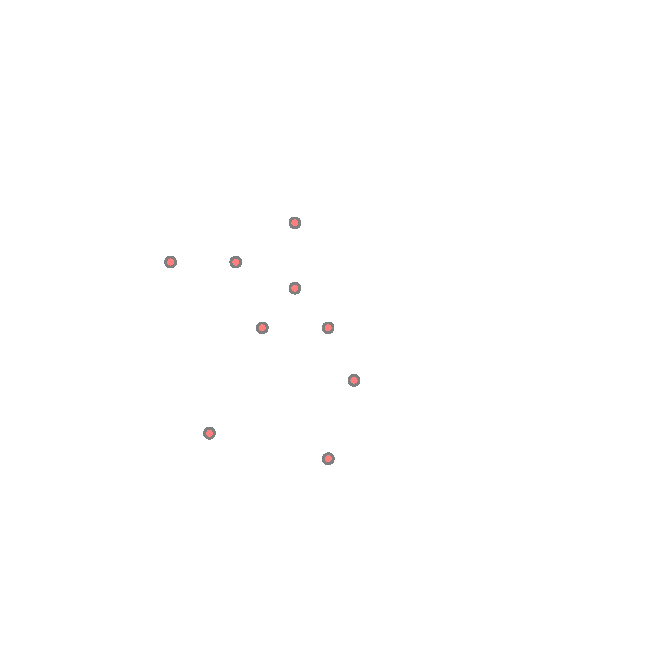
\includegraphics[height = 1.7in]{test_sample.tikz}
      %                 \label{fig:test}}
      %                 \subfloat[]{\includegraphics[height = 1.7in]{plsim_153.tikz}
      %                 \label{fig:sim_lo}}
      %                 \subfloat[]{\includegraphics[height = 1.7in]{plsim_75.tikz}
      %                 \label{fig:sim_hi}}
      %                 \caption{(a) Sample distribution. Simulation of the reconstructed sample image at: (b) $\Re k_{\p} = 39.5$ (c) $\Re k_{\p} = 80$}
      %                 \label{fig:simulation}
      %               \end{figure}
      %             \end{frame}
      %             % ------------------------------------------------------------
      %             % ------------------------------------------------------------
      %             % ------------------------------------------------------------
      %             % ------------------------------------------------------------
      %             % ------------------------------------------------------------
      %             % ------------------------------------------------------------
      %             % ------------------------------------------------------------
      %             % ------------------------------------------------------------
      %             % ------------------------------------------------------------
      %             % ------------------------------------------------------------
      %             % ------------------------------------------------------------
      %             % ------------------------------------------------------------
      %             % ------------------------------------------------------------
      %             % ------------------------------------------------------------
      %             % ------------------------------------------------------------
      %             % ------------------------------------------------------------
      %             % ------------------------------------------------------------
      %             % ------------------------------------------------------------
      %             % ------------------------------------------------------------
      %             % ------------------------------------------------------------
      %             % ------------------------------------------------------------
      %             \section{Conclusion}
      %             \begin{frame}
      %               \frametitle{Summary}
      %               \framesubtitle{Two-dimensional plasmonic devices}
      %               \begin{itemize}
      %                 \item Subwavelength wave phenomena at optical and terahertz frequencies
      %                 \item Realization of terahertz sources and sensors
      %                 \item 2D nature of waves permits subwavelength confinement
      %                 \item Plasmonic activity
      %                 \item Nanoscale imaging using terahertz plasma waves
      %               \end{itemize}
      %             \end{frame}
      %             % ------------------------------------------------------------
      %             % ------------------------------------------------------------
      %             % ------------------------------------------------------------
      %             % ------------------------------------------------------------
      %             % ------------------------------------------------------------
      %             % ------------------------------------------------------------
      %             % ------------------------------------------------------------
      %             \begin{frame}
      %               \frametitle{Acknowledgements}
      %               \framesubtitle{Sponsorship}
      %               \begin{itemize}
      %                 \item The Fulbright Program
      %               \end{itemize}
      %               \begin{figure}
      %                 \centering
      %                 \def\svgwidth{.4\linewidth}
      %                 \input{figures/fulbright.pdf_tex}
      %                 % \caption{(a). Actual and its equivalent models for the (b) external and, (c) Internal region }
      %               \end{figure}
      %             \end{frame}
      %             % ------------------------------------------------------------
      %             % ------------------------------------------------------------
      %             % ------------------------------------------------------------
      %             % ------------------------------------------------------------
      %             % ------------------------------------------------------------
      %             % ------------------------------------------------------------
      %             % ------------------------------------------------------------
      %             \begin{frame}[plain,c]
      %               \begin{center}
      %                 \Huge Thank you!
      %               \end{center}
      %             \end{frame}
      %             % ------------------------------------------------------------
      %             % ------------------------------------------------------------
      %             % ------------------------------------------------------------
      %             % ------------------------------------------------------------
      %             % ------------------------------------------------------------
      %             % ------------------------------------------------------------
      %             % ------------------------------------------------------------
      %             \begin{frame}[plain,c]
      %               \begin{center}
      %                 \Huge Questions?
      %               \end{center}
      %             \end{frame}
                  \end{document}
